\section{Security Analysis}
\label{sec:security}

The rest of this section describes the security properties of
enclaves, discussing the trade-offs made while trying to balance security with
backwards compatibility.

% ECREATE forces R, W, X to 0 in the page's EPCM. EADD also forces R/W/X to 0
% if the page type in SECINFO is PT_TCS (the only special type it can create).
%
%
% EPA doesn't read any SECINFO, and uses 0 for R, W, X.

% ERESUME can be replaced by normal EENTER, XRESTOR and accounting. Describe
% and argue against ERESUME.


% The use of the page version (nonce) as counter in AES-GCM makes it impossible
% for malicious system software to determine whether an EPC page's contents has
% changed between two evictions.
% However, the dirty bit in the EPC page's PTE will leak that information.

% According to the ECREATE pseudo-code in the Intel manual, EIDs are assigned
% using a counter that is atomically incremented on every ECREATE. This makes
% the field predictible to system software.


% The SGX instruction that evicts an EPC page, EWB, ensures that the VA slot it
% is supposed to write is unused.
% The VA unused slot check in EWB is unnecessary. Bad system software can only
% overwrite a version and impair its ability to restore a page.

Enclaves were designed to contain and protect the privacy-sensitive parts of an
application. All the code that handles private data must receive integrity
protection. Otherwise, a hostile environment could modify the code to leak
information about private data. Therefore, the SGX programming model prescribes
that code which accesses private data must be entirely contained inside an
enclave. Jumping into and out of enclave code must be performed explicitly
using the dedicated instructions \texttt{EENTER} and \texttt{EEXIT}.



\begin{figure}[hbt]
  \centering
  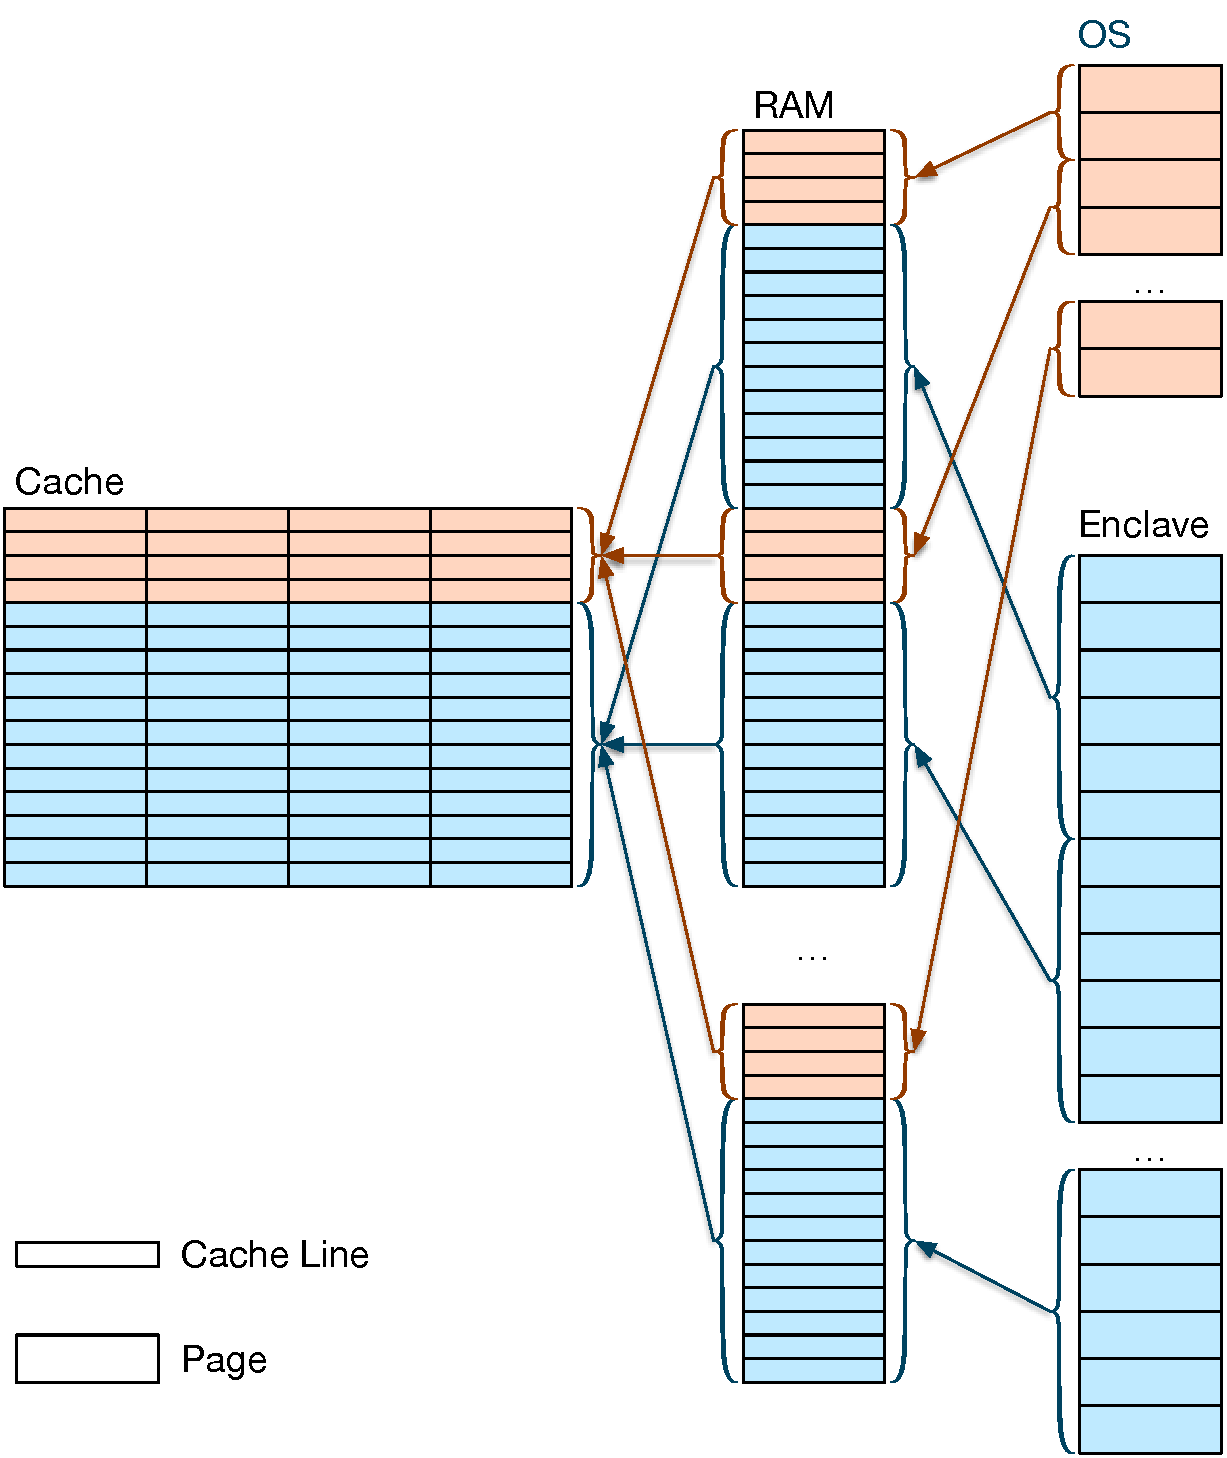
\includegraphics[width=85mm]{figures/cache_partitions.pdf}
  \caption{
    Cache partitioning between two applications. Each application has some
    cache sets allocated to it, and only uses RAM regions that map to its cache
    sets. When partitioning the L1 cache, applications have to follow this
    constraint themselves. When the L2 cache is partitioned, the OS can map the
    pages in an application's virtual address space to the RAM regions that the
    application can use, so applications are oblivious to the cache
    partitioning.
  }
  \label{fig:cache_partitions}
\end{figure}
